\section{Adversarial Example Landscape}
\transitionFrame{Adversarial Example Landscape}

\begin{frame}{Investigating the ``Inner Maximization''}
  \onslide<+->{%
    \begin{equation}
      \min_{\params} \rho(\params) \text{, where } \rho(\params) = \mathbb{E}_{(\X,\y) \sim \distr} \sbrack{\red{\max_{\delta \in \sPerturb} \loss (\X + \perturb, \y ; \params)}}
    \end{equation}
  }

  \begin{itemize}[<+->]
    \setlength{\itemsep}{20pt}
    \item Preceding theoretical analysis of \textbf{\red{inner maximization}} described PGD's usefulness to provide guarantees regarding first-order adversaries
    \item \textbf{Goal of this Section}: Demonstrate \textit{empirically} that the theoretical analysis holds even in environments that are theoretically \textit{intractable}
      \begin{itemize}[<+->]
        \setlength{\itemsep}{8pt}
        \item \textbf{Recall}: Inner maximization is highly \textit{non-concave} and not continuously-differentiable
        \item \textbf{Question}: Why are we interested in concavity and not convexity?
      \end{itemize}
  \end{itemize}
\end{frame}


\begin{frame}{Experimental Setup}
  \onslide<+->{Setup applies for all experiments in this section}
  \begin{itemize}[<+->]
    \setlength{\itemsep}{10pt}
    \item \textbf{Datasets}: MNIST \& CIFAR10

    \item \textbf{Procedure}: Select example,~$\X$, u.a.r.\ from the dataset, then for each random restart:
      \begin{enumerate}[<+->]
        \setlength\itemsep{6pt}
        \item Select initial perturbation,~${\perturb \in \sPerturb}$, u.a.r.
        \item Perform PGD on perturbed example, ${\X + \perturb}$
      \end{enumerate}

    \item \textbf{\# Random Restarts}: Varies by experiment

    \item \textbf{Loss Function}: Cross-entropy
      \onslide<+->{
        \begin{equation}\label{eq:CrossEntropy}
          \loss(y,\hat{y}) = \sum_{c \in \mathcal{C}} -y_c \log \left( \hat{y}_{c} \right)
        \end{equation}
      }
  \end{itemize}
\end{frame}


\begin{frame}{Experiment~\#1: $\Delta\loss$ vs.\ \#Iterations}
  \onslide<+->{\textbf{Goal}: Study change in adversarial loss for each iteration of PGD}
  \begin{itemize}[<+->]
    \item \textbf{\# Random Restarts}: 20
  \end{itemize}

  \begin{columns}
    \begin{column}{0.23\textwidth}
      \begin{center}
        \onslide<+->{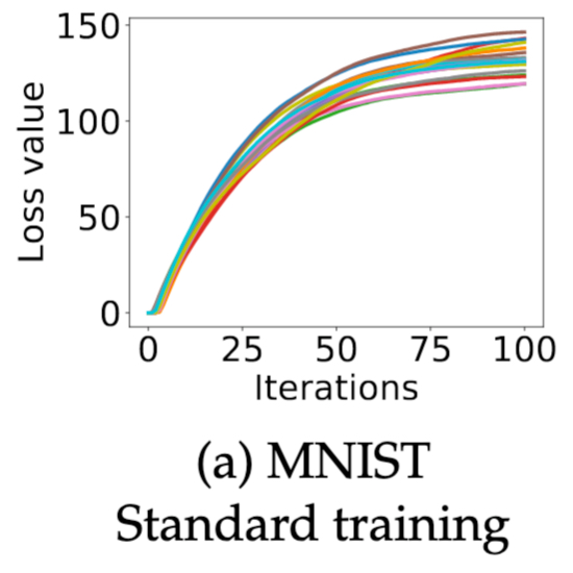
\includegraphics[scale=0.32]{loss_v_iter/mnist_standard.pdf}}
      \end{center}
    \end{column}
    \begin{column}{0.2\textwidth}
      \begin{center}
        \onslide<+->{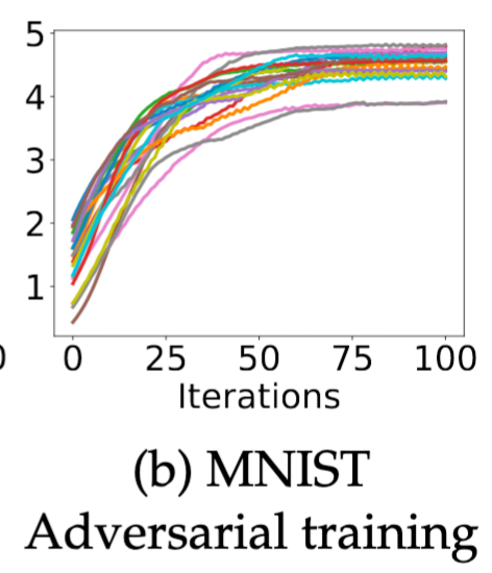
\includegraphics[scale=0.32]{loss_v_iter/mnist_adv.pdf}}
      \end{center}
    \end{column}
    \begin{column}{0.21\textwidth}
      \begin{center}
        \onslide<+->{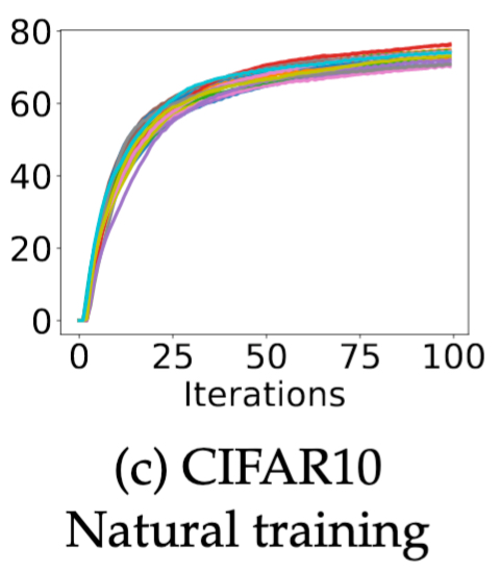
\includegraphics[scale=0.32]{loss_v_iter/cifar_standard.pdf}}
      \end{center}
    \end{column}
    \begin{column}{0.22\textwidth}
      % \vspace{-9pt}
      \begin{center}
        \onslide<+->{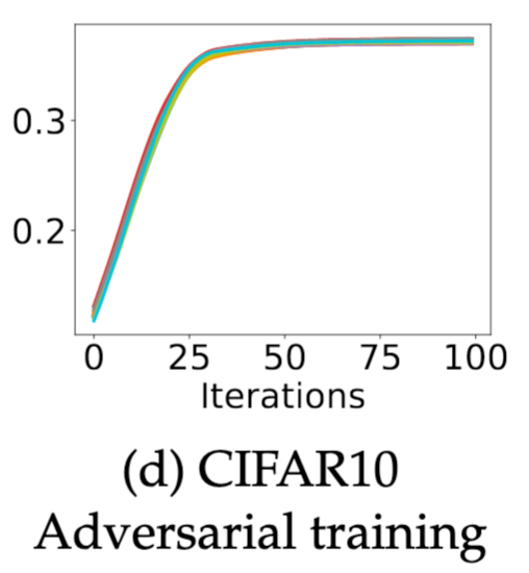
\includegraphics[scale=0.32]{loss_v_iter/cifar_adv.pdf}}
      \end{center}
    \end{column}
  \end{columns}
  \vfill
  \onslide<+->{\green{\textbf{Takeaways}}}
  \begin{itemize}[<+->]
    \item Adversarial training significantly reduces loss on adversarial examples.
    \item Loss values are \textbf{\blue{well-concentrated}}
      \begin{itemize}
        \item Echoes \textit{folklore belief} that neural network training possible since many local minima with similar loss values
      \end{itemize}
  \end{itemize}
\end{frame}


\begin{frame}{Experiment~\#2: Absence of Outliers}
  \onslide<+->{\textbf{Goal}: Verify security guarantee across many examples \& random restarts}
  \begin{itemize}[<+->]
    \item \textbf{\# Examples} ($x$): 5
    \item \textbf{\# Random Restarts}: 100K
  \end{itemize}

  \vspace{-15pt}
  \begin{columns}
    \begin{column}{0.7\textwidth}
      \begin{center}
        \onslide<4->{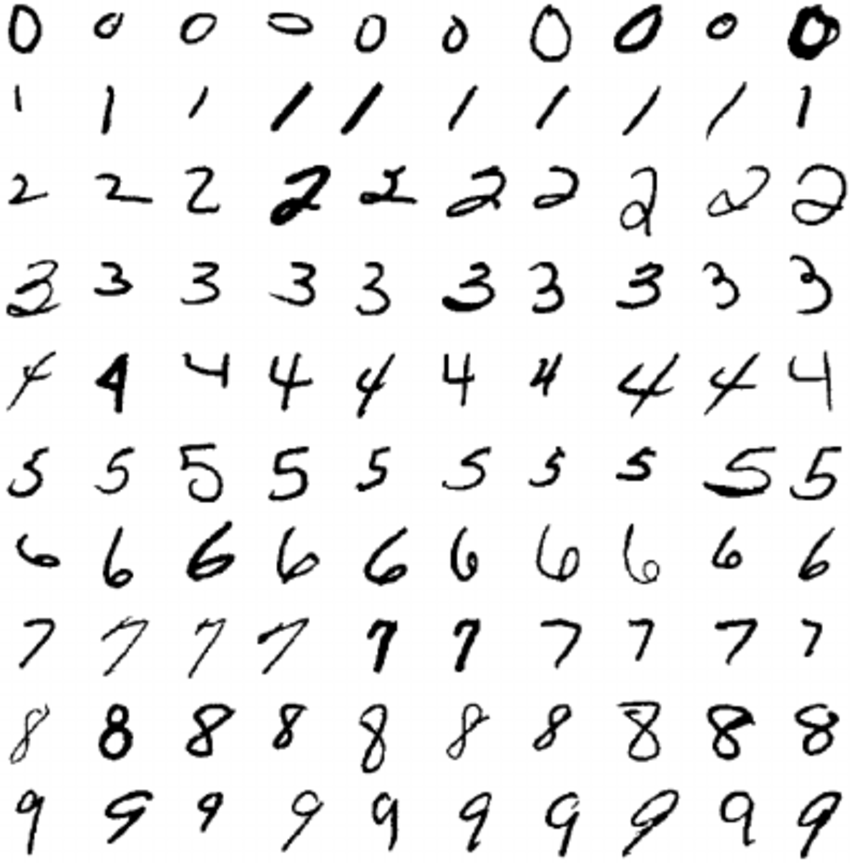
\includegraphics[scale=0.19]{loss_hist/mnist}}

        \onslide<6->{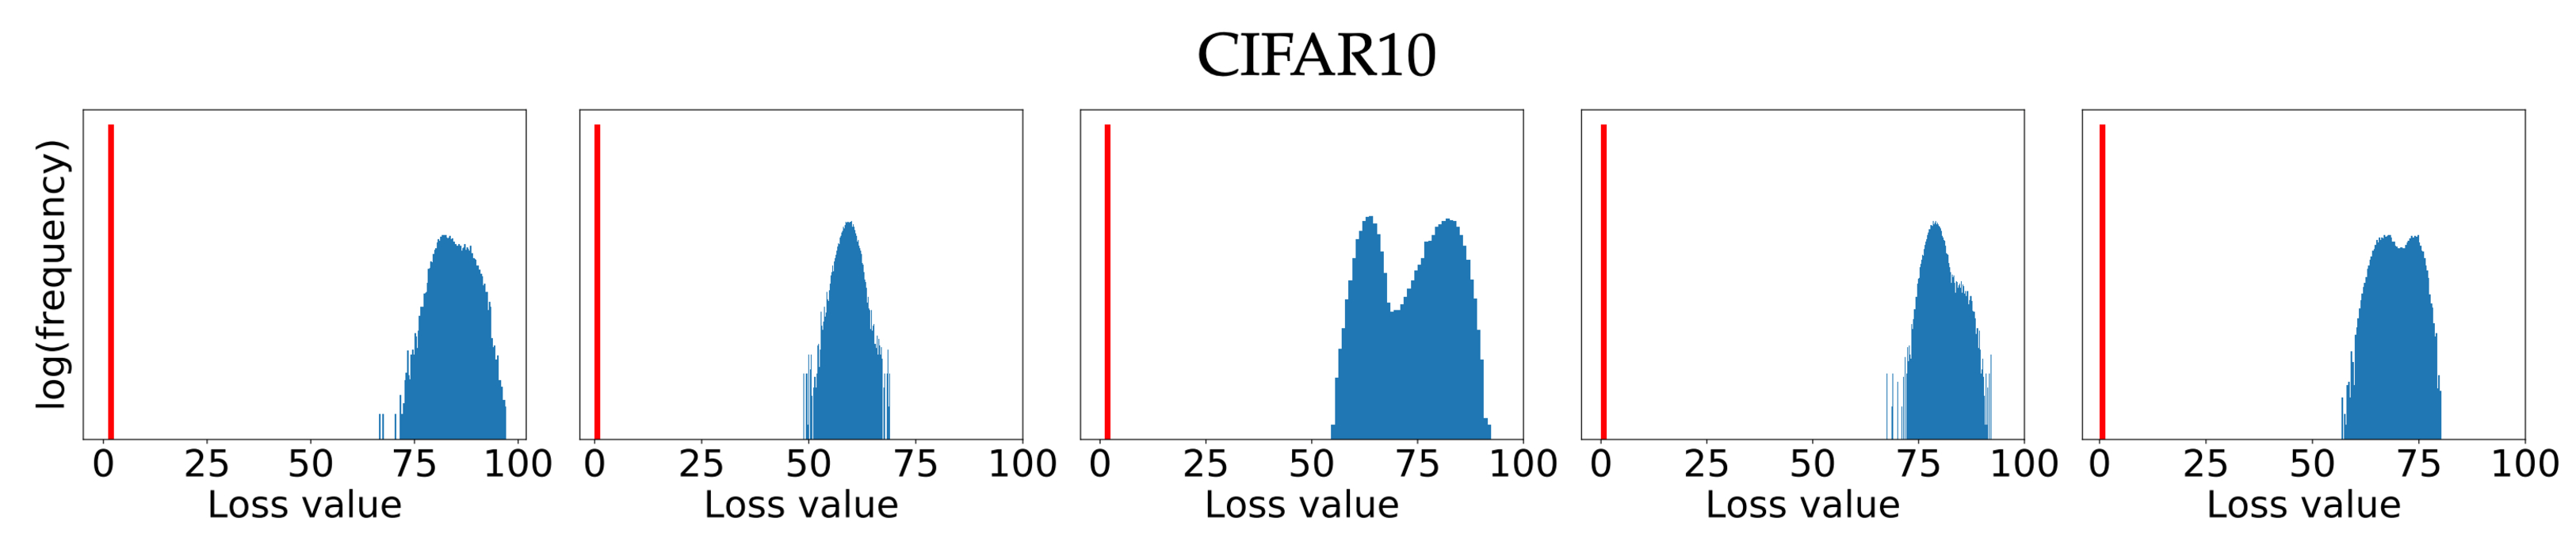
\includegraphics[scale=0.19]{loss_hist/cifar}}
      \end{center}
    \end{column}
    \begin{column}{0.25\textwidth}
      \vspace{20pt}
      \onslide<5->{
        \begin{itemize}
          \setlength{\itemsep}{20pt}
          \item \textbf{\blue{Blue}}: Standard training
          \item \textbf{\red{Red}}: Adversarial training
        \end{itemize}
      }
    \end{column}
  \end{columns}

  \vfill
  \onslide<7->{\green{\textbf{Takeaway}}: No outliers (i.e., high loss adversarial examples) \& concentrated losses}
\end{frame}


\begin{frame}{Experiment~\#3: ``Mode Collapse''}
  \onslide<+->{\textbf{\blue{Mode Collapse}}: Common problem in GANs where the generated outputs have limited diversity.}
  \vfill
  \onslide<+->{\textbf{Goal}: Demonstrate that the generated adversarial examples are noticeably distinct:}
  \begin{itemize}[<+->]
    \item \textbf{\# Random Restarts}: 10,000
    \item \textbf{Metric}: Inter-adversarial example (Euclidean) distance
  \end{itemize}
  \vfill
  \onslide<+->{\textbf{\green{Result}}: Inter-maxima distance is distributed close to the expected distance between \textit{two random points} in the $\ell_{\infty}$\-/ball and cosine similarity between points is close to 90\textsuperscript{$\circ$}.}
  \begin{itemize}[<+->]
    % \item Empirically demonstrates no adversarial example ``mode collapse''
    \item Recall the ``curse of dimensionality'' so take with a grain of salt
  \end{itemize}
  \vfill
  \onslide<+->{\textbf{\green{Takeaway}}: No evidence of mode collapse}
\end{frame}
